\documentclass[tikz,border=8pt]{standalone}
% Shared look for every TikZ diagram. Load with \input{../../tools/tikz-style.tex}
\usepackage[T1]{fontenc}
\usepackage{lmodern}
\renewcommand{\sfdefault}{lmr}  % diagrams use the same serif as the text
\usetikzlibrary{arrows.meta, positioning, shapes.geometric, calc, fit, backgrounds}
\definecolor{cblue}{HTML}{4C78A8}
\definecolor{corange}{HTML}{F58518}
\definecolor{cgreen}{HTML}{54A24B}
\definecolor{cred}{HTML}{E45756}
\definecolor{cpurple}{HTML}{B279A2}
\definecolor{cgrey}{HTML}{6B6B6B}
\tikzset{
  every picture/.style={font=\sffamily, line width=1.2pt},
  box/.style={draw=#1, fill=#1!12, rounded corners=4pt, align=center, inner sep=7pt, minimum height=1.1cm},
  box/.default=cgrey,
  arrow/.style={-{Stealth[length=3mm]}, draw=cgrey, line width=1.4pt},
  title/.style={font=\sffamily\bfseries\Large},
  note/.style={font=\sffamily\small, text=cgrey, align=center},
}
\AtBeginDocument{\hyphenpenalty=10000 \exhyphenpenalty=10000}

\begin{document}
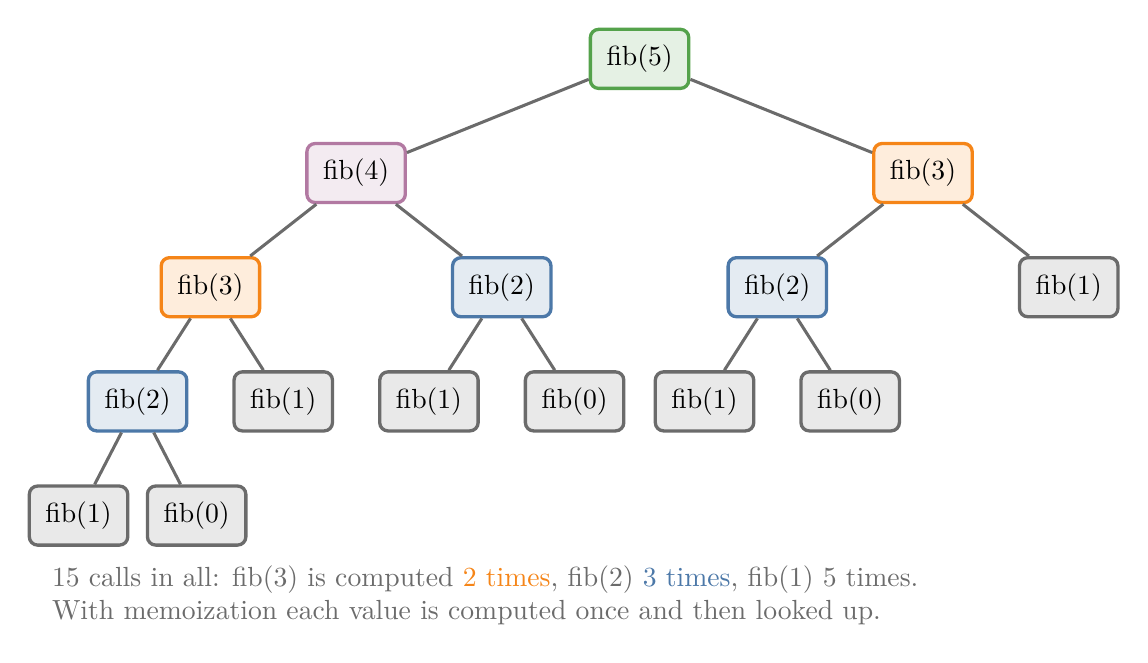
\begin{tikzpicture}[
  f/.style={draw=#1, fill=#1!15, rounded corners=3pt, minimum width=1.25cm, minimum height=0.75cm, font=\sffamily, line width=1.2pt},
  f/.default=cgrey,
  level distance=1.45cm, edge from parent/.style={draw=cgrey, line width=1.1pt},
  level 1/.style={sibling distance=7.2cm}, level 2/.style={sibling distance=3.7cm},
  level 3/.style={sibling distance=1.85cm}, level 4/.style={sibling distance=1.5cm}]
  \node[f=cgreen] {fib(5)}
    child {node[f=cpurple] {fib(4)}
      child {node[f=corange] {fib(3)}
        child {node[f=cblue] {fib(2)} child {node[f] {fib(1)}} child {node[f] {fib(0)}}}
        child {node[f] {fib(1)}}}
      child {node[f=cblue] {fib(2)} child {node[f] {fib(1)}} child {node[f] {fib(0)}}}}
    child {node[f=corange] {fib(3)}
      child {node[f=cblue] {fib(2)} child {node[f] {fib(1)}} child {node[f] {fib(0)}}}
      child {node[f] {fib(1)}}};
  \node[note, font=\sffamily\normalsize, align=left, anchor=north west] at (-7.6, -6.3)
    {15 calls in all: fib(3) is computed {\color{corange}2 times}, fib(2) {\color{cblue}3 times}, fib(1) 5 times.\\
     With memoization each value is computed once and then looked up.};
\end{tikzpicture}
\end{document}
